\documentclass[12pt]{article} \usepackage{url, graphicx}

% page layout
\setlength{\topmargin}{-0.25in}
\setlength{\textheight}{9.5in}
\setlength{\headheight}{0in}
\setlength{\headsep}{0in}

% problem formatting
\newcommand{\problemname}{Problem}
\newcounter{problem}

% math
\newcommand{\dd}{\mathrm{d}}

% primary units
\newcommand{\rad}{\mathrm{rad}}
\newcommand{\kg}{\mathrm{kg}}
\newcommand{\m}{\mathrm{m}}
\newcommand{\s}{\mathrm{s}}

% secondary units
\renewcommand{\deg}{\mathrm{deg}}
\newcommand{\km}{\mathrm{km}}
\newcommand{\mi}{\mathrm{mi}}
\newcommand{\h}{\mathrm{h}}
\newcommand{\ns}{\mathrm{ns}}
\newcommand{\J}{\mathrm{J}}
\newcommand{\eV}{\mathrm{eV}}
\newcommand{\W}{\mathrm{W}}

% derived units
\newcommand{\mps}{\m\,\s^{-1}}
\newcommand{\mph}{\mi\,\h^{-1}}
\newcommand{\mpss}{\m\,\s^{-2}}

% random stuff
\sloppy\sloppypar\raggedbottom\frenchspacing\thispagestyle{empty}

\begin{document}

\noindent
Name: \rule[-1ex]{0.55\textwidth}{0.1pt}
NetID: \rule[-1ex]{0.2\textwidth}{0.1pt}

\section*{NYU Physics I---Term Exam 5}

\paragraph{\problemname~\theproblem:}\refstepcounter{problem}%
What is the difference in pressure (in Pa) between a point $1\,\m$
below the surface of the ocean and a point $3\,\m$ below the surface?
(From Lecture on 2016-11-03.)

\vfill

\paragraph{\problemname~\theproblem:}\refstepcounter{problem}%
If rolled (without slipping) down a plane, with a fair start (at
rest), which would win a gravity-driven race, a solid, uniform sphere
of mass $0.9\,\kg$ and radius $0.05\,\m$ or a solid, uniform cylinder
of mass $0.4\,\kg$ and radius $0.01\,\m$? No calculation required, but
say \emph{why, in less than 30 words}. Box your answer. (From Lecture
on 2016-11-10.)

\vfill

\paragraph{\problemname~\theproblem:}\refstepcounter{problem}%
A blimp has a volume of $7000\,\m^3$ of He (atomic mass 4) at STP,
floating in air (atomic mass around 28) at STP. How much mass in $kg$
can the blimp carry, roughly? That mass will include the skin, the
cabin, the motors, the crew and cargo! (From Problem Set 9.)

\vfill
~
\clearpage

\paragraph{\problemname~\theproblem:}\refstepcounter{problem}%
A spinning figure skater (subject to no net external torque)
reduces her moment of inertia by a factor
of 1.5 (that is $I_{\mathrm{new}} = I_{\mathrm{old}} / 1.5$). By
what factor does her kinetic energy change? Does it increase or
decrease or stay the same?
(From Problem Set 10.)

\vfill

\paragraph{\problemname~\theproblem:}\refstepcounter{problem}%
Imagine that the rate at which particles hit a wall is $\Gamma$
(number per unit time).  Imagine that each of these particles has mass
$m$ and hits the wall with a normal velocity of $v$ (that is, the
component of the velocity perpendicular to the wall is $v$). What is
the mean force on the wall? Collisions are elastic. (From the
recitation on the ideal gas.)

\vfill

\paragraph{\problemname~\theproblem:}\refstepcounter{problem}%
The truck is accelerating to the right at acceleration $a$, and the
pipe is not tied down. Draw a free body diagram for the pipe, assuming static friction. Imagine
(despite how the figure is drawn) that the pipe is not touching the
cab of the truck, it is only touching the bed (floor) of the truck. (From the
recitation on rolling.)\\ \rule{0.3\textwidth}{0pt}
\resizebox{0.4\textwidth}{!}{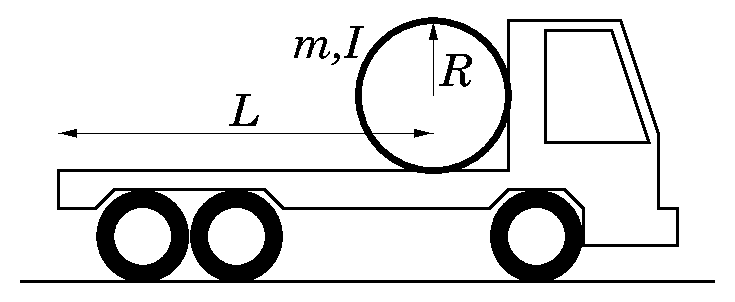
\includegraphics{truckpipe.eps}}

\vfill
~
\end{document}
